\section{实验:组成串联电路和并联电路}\label{sec:7-8}

在这个实验里,我们要自己动手连接简单的电路,学习和掌握串联、并联这两种最基本的电路连接方法。

我们要连接的是图 \ref{fig:7-25} 和图 \ref{fig:7-26} 所示的电路。
需要哪些器材(包括名称和数量),自己可以根据图列出清单,再按清单检查实验桌上的器材是否够用。

(1) 组成串联电路

接照图 \ref{fig:7-25} 组成串联电路。
连接电路的时候应该按照一定的顺序,这个顺序可以自己定,
例如可以顺着电流的方向从电池组的正极开始接线,再依次接好电键 $K$、灯 $L_1$、灯 $L_2$,最后连接电池组的负极,
也可以逆着电流的方向从电池组负极开始接线,依次接好 $L_2$、$L_1$、$K$,最后连接电池组正极。
必须注意,在连接电路的过程中,电键应该是断开的。

电路接好后,先闭合再断开电键,观察串联电路里的电键是同时控制两个灯泡,还是只控制其中一个。

把电键 $K$ 改接到 $L_1$ 和 $L_2$ 之间,再改接到 $L_2$ 和电池组负极之间,
每一次都闭合、断开电键,观察电键的控制作用是否改变了。

分别画出上面三次实验的电路图,在图旁记下观察结果。
根据上面的实验回答;串联电路里的电键是同时控制两个灯泡,还是只控制其中一个?
在串联电路里,电键的位置改变了,它的作用有没有改变?

\begin{figure}[htbp]
    \centering
    \begin{minipage}{7cm}
    \centering
    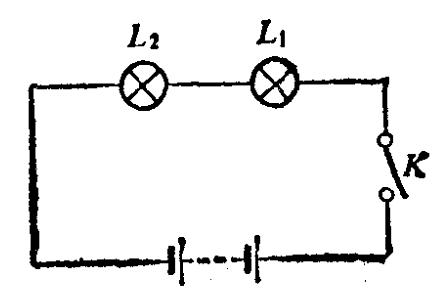
\includegraphics[width=6cm]{../pic/czwl2-ch7-25}
    \caption{}\label{fig:7-25}
    \end{minipage}
    \qquad
    \begin{minipage}{7cm}
    \centering
    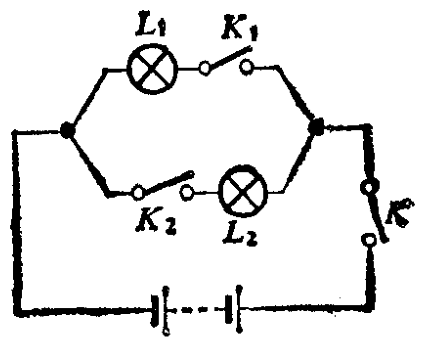
\includegraphics[width=6cm]{../pic/czwl2-ch7-26}
    \caption{}\label{fig:7-26}
    \end{minipage}
\end{figure}


(2) 组成并联电路

照图 \ref{fig:7-26} 组成并联电路。把三个电键都闭合,然后进行下述观察:

断开、闭合干路电键 $K$,观察它控制哪个灯泡;

断开、闭合支路电键 $K_1$,观察它控制哪个灯泡;

断开、闭合支路电键 $K_2$,观察它控制哪个灯泡。

根据上面的观察回答:在并联电路里,干路中的电键和各支路中的电键,它们的作用有什么不同?


\lianxi

(1) 马路上的路灯如果有一盏坏了(例如灯丝断了),其他的灯还能照常亮。
根据这个现象你能不能判断出路灯是串联的还是并联的?为什么?

(2) 画出图 \ref{fig:7-27} 所示电路的电路图。

\begin{figure}[htbp]
    \centering
    \begin{minipage}{5cm}
    \centering
    \vspace{2cm}
    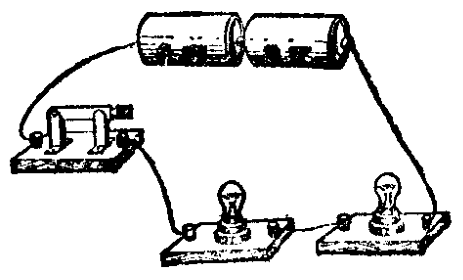
\includegraphics[width=5cm]{../pic/czwl2-ch7-27}
    \caption{}\label{fig:7-27}
    \end{minipage}
    \qquad
    \begin{minipage}{11cm}
    \centering
    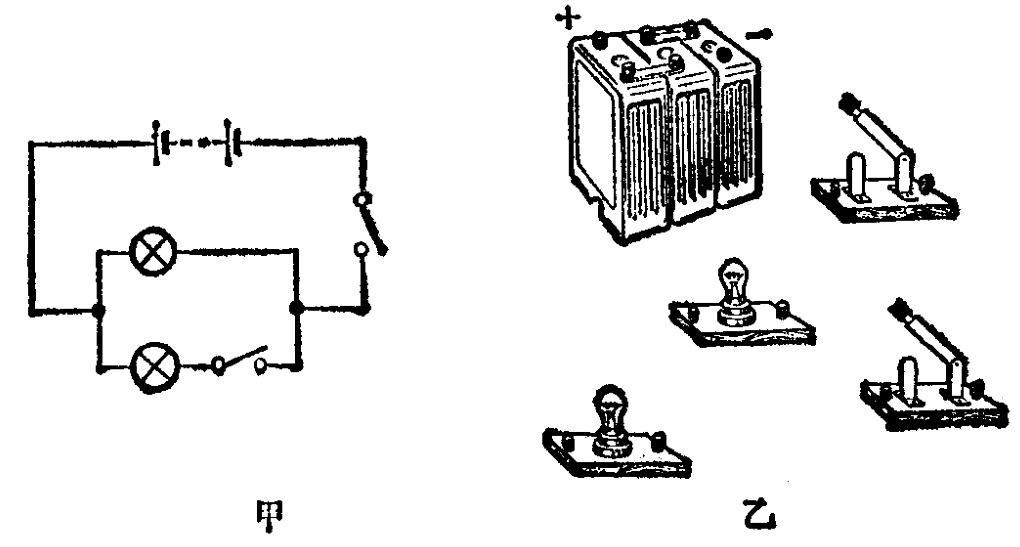
\includegraphics[width=10cm]{../pic/czwl2-ch7-28}
    \caption{}\label{fig:7-28}
    \end{minipage}
\end{figure}

(3) 按照图 \ref{fig:7-28} 甲的电路图,将图乙中的元件连成电路(元件位置不动,用铅笔线代替连接用的导线)。

(4) 有三盏电灯,想把它们连接在一个电路里,并且开关每盏电灯时不影响别的灯,应该怎样连接?画一个电路图表示出来。

(5) 在图 \ref{fig:7-29} 所示的电路中:

\begin{figure}[htbp]
    \centering
    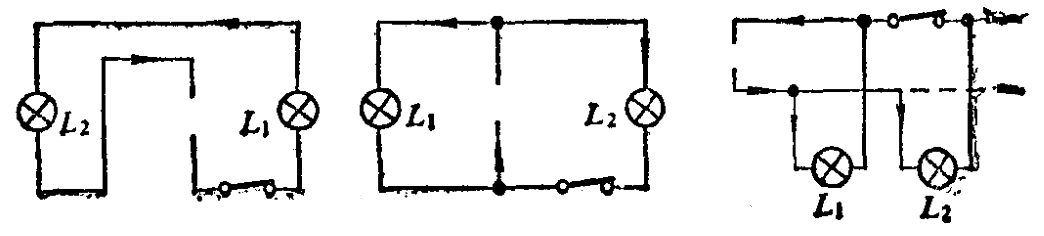
\includegraphics[width=0.7\textwidth]{../pic/czwl2-ch7-29}
    \caption{}\label{fig:7-29}
\end{figure}

\tc{1} 根据标出的电流方向,把电池组填进电路;

\tc{2} 电灯 $L_1$ 和 $L_2$ 是怎样连接的?把并联电路的干路部分用色笔描一下;

\tc{3} 如果把电键断开,各灯还能发光吗?



\section*{小实验}

\begin{figure}[htbp]
    \centering
    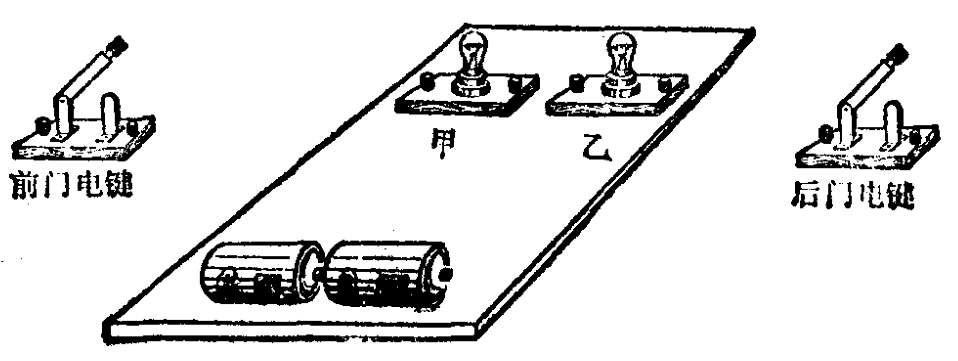
\includegraphics[width=0.7\textwidth]{../pic/czwl2-ch7-30}
    \caption{}\label{fig:7-30}
\end{figure}

图 \ref{fig:7-30} 中的木板上装着甲、乙两个小电灯和一个电池组。
假定这块木板安装在学校传达室里,学校传达室的值班人员,想从甲灯亮或乙灯亮,
知道是前门来人闭合前门电键,还是后门来人闭合后门电键。
要求这两个灯共用一个电池组。
请你替值班人员设计出符合他需要的电路,画出电路图,
再按照电路图把图 \ref{fig:7-30} 中的实物连接起来,并试验一下这个电路是否符合需要。

